\part{Graphs}
\frame{\partpage}

\begin{frame}{Graphs}
	\begin{columns}
		\pause
		\begin{column}{0.3\textwidth}
			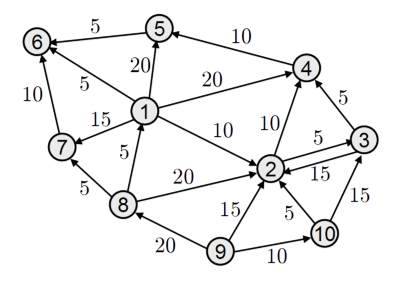
\includegraphics[width=\textwidth]{graph1}
			\par
			\vspace{2ex}
			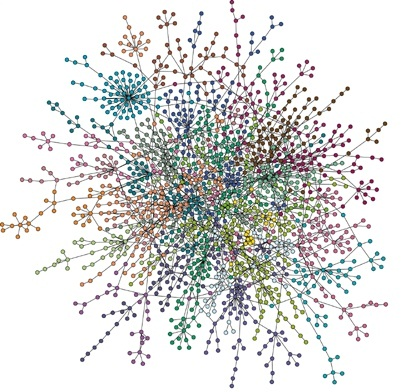
\includegraphics[width=\textwidth]{graph2}
		\end{column}
		\begin{column}{0.68\textwidth}
			\begin{itemize}
				\pause\item A \textbf{graph} is defined by:
					\begin{itemize}
						\pause\item A collection of \textbf{nodes} or \textbf{vertices} (points)
						\pause\item A collection of \textbf{edges} or \textbf{arcs} (lines or arrows between points)
					\end{itemize}
				\pause\item Often used to model \textbf{networks} (e.g.\ social networks, transport networks, game levels, automata, ...)
				\pause\item \textbf{Directed} graph: edges are arrows
				\pause\item \textbf{Undirected} graph: edges are lines
			\end{itemize}
		\end{column}
	\end{columns}
\end{frame}

\begin{frame}{Implementing graphs}
	\begin{itemize}
		\pause\item A graph is a \textbf{collection of nodes}
		\pause\item Each node has a \textbf{collection of edges}
		\pause\item Each edge has exactly \textbf{two nodes} associated with it
	\end{itemize}
\end{frame}

\begin{frame}{Trees}
	\begin{columns}
		\pause
		\begin{column}{0.3\textwidth}
			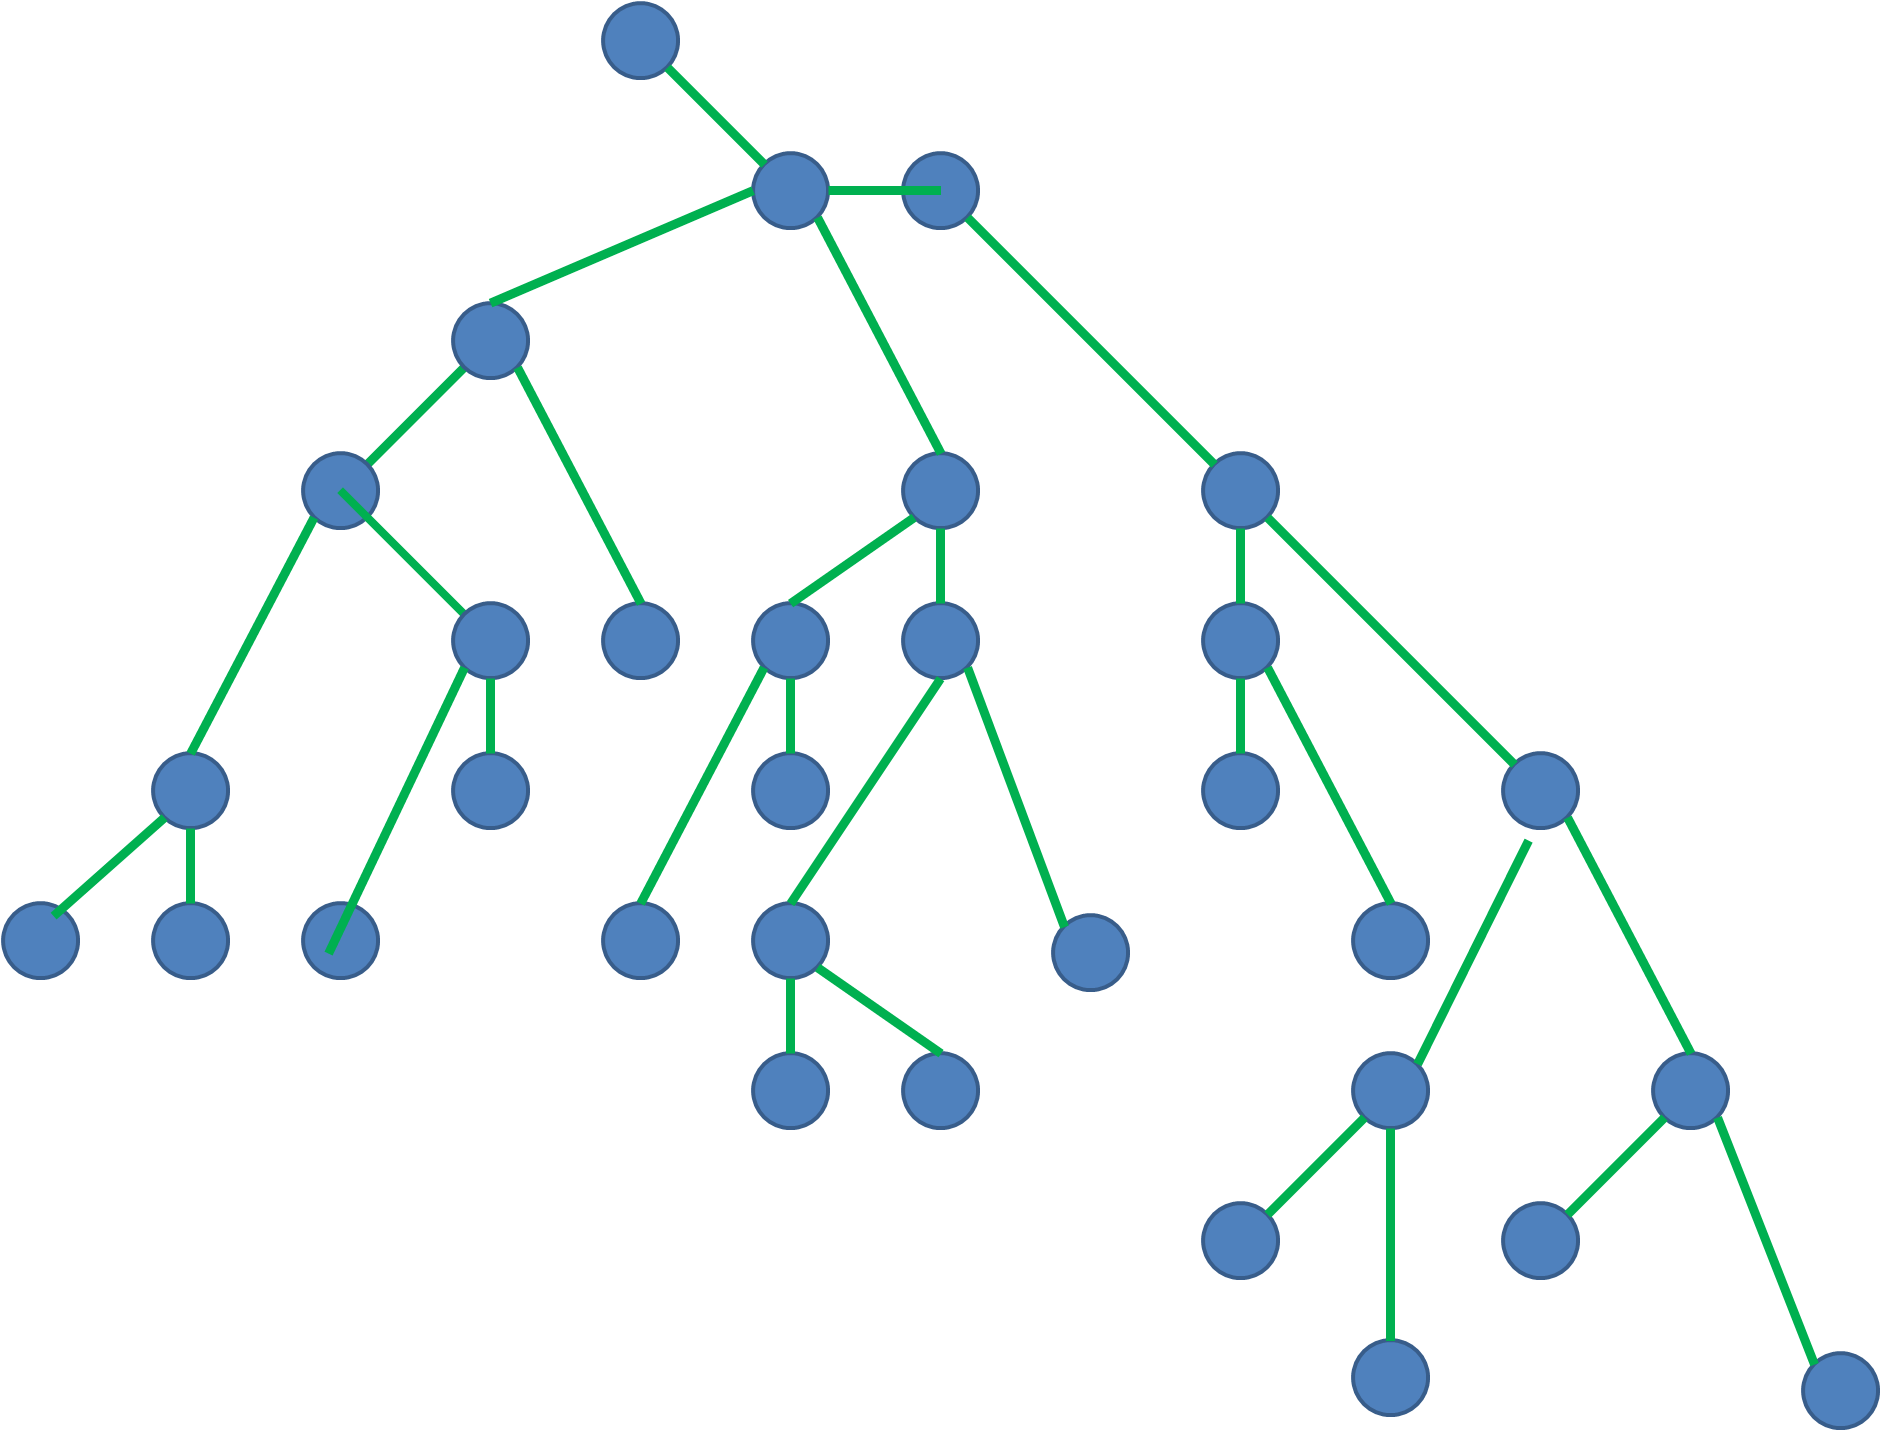
\includegraphics[width=\textwidth]{tree2}
			\par
			\vspace{2ex}
			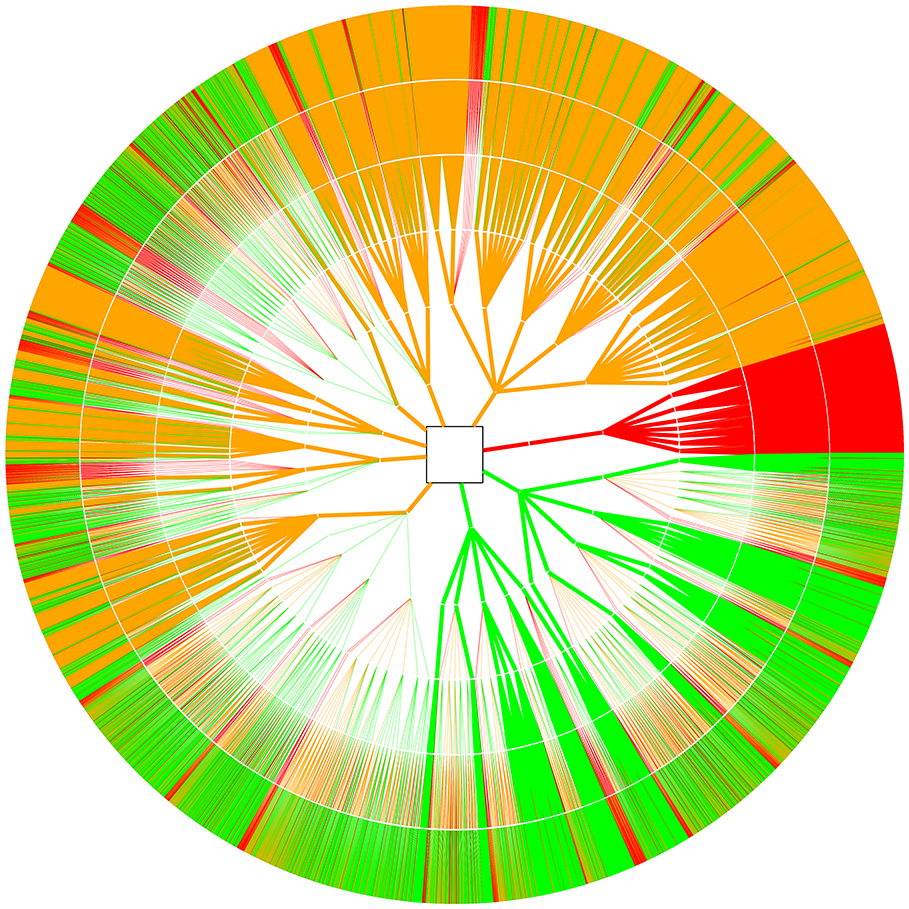
\includegraphics[width=\textwidth]{tree}
		\end{column}
		\begin{column}{0.68\textwidth}
			\begin{itemize}
				\pause\item A \textbf{tree} is a special type of directed graph where:
					\begin{itemize}
						\pause\item One node (the \textbf{root}) has no incoming edges
						\pause\item All other nodes have exactly 1 incoming edge
					\end{itemize}
				\pause\item Edges go from \textbf{parent} to \textbf{child}
					\begin{itemize}
						\pause\item All nodes except the root have exactly one parent
						\pause\item Nodes can have 0, 1 or many children
					\end{itemize}
				\pause\item Used to model \textbf{hierarchies} (e.g.\ file systems, object inheritance, scene graphs, state-action trees, ...)
			\end{itemize}
		\end{column}
	\end{columns}
\end{frame}

\begin{frame}{Implementing trees}
	\begin{itemize}
		\pause\item A graph has a \textbf{root node}
		\pause\item Each node has a \textbf{collection of children}
		\pause\item Each node other than the root has a \textbf{single parent}
	\end{itemize}
\end{frame}

\begin{frame}{Tree traversal}
	\begin{itemize}
		\pause\item \textbf{Traversal}: visiting all the nodes of the tree
		\pause\item Two main types
			\begin{itemize}
				\pause\item Depth first
				\pause\item Breadth first
			\end{itemize}
	\end{itemize}
\end{frame}

\begin{frame}{Tree traversal}
	\pause\footnotesize
%	\begin{columns}
%		\begin{column}{0.48\textwidth}
			\begin{algorithmic}
				\Procedure{DepthFirstSearch}{} \pause
					\State let $S$ be a stack \pause
					\State push root node onto $S$ \pause
					\While{$S$ is not empty} \pause
						\State pop $n$ from $S$ \pause
						\State print $n$ \pause
						\State push children of $n$ onto $S$ \pause
					\EndWhile
				\EndProcedure
			\end{algorithmic}
%		\end{column}
		\pause
%		\begin{column}{0.48\textwidth}
		\vspace{2ex}
			\begin{algorithmic}
				\Procedure{BreadthFirstSearch}{} \pause
					\State let $Q$ be a queue \pause
					\State enqueue root node into $Q$ \pause
					\While{$Q$ is not empty} \pause 
						\State dequeue $n$ from $Q$ \pause
						\State print $n$ \pause
						\State enqueue children of $n$ into $Q$ \pause
					\EndWhile
				\EndProcedure
			\end{algorithmic}
%		\end{column}
%	\end{columns}
\end{frame}

\begin{frame}{Recursive depth first search}
	\pause
	\begin{algorithmic}
		\Procedure{DepthFirstSearch}{$n$} \pause
			\State print $n$ \pause
			\For{\textbf{each} child $c$ of $n$} \pause
				\State \Call{DepthFirstSearch}{$c$} \pause
			\EndFor
		\EndProcedure
	\end{algorithmic}
	\begin{itemize}
		\pause\item Compare to the pseudocode on the previous slide. Where is the stack?
	\end{itemize}
\end{frame}

\begin{frame}{Tree traversal example}
	\begin{center}
		Socrative \texttt{FALCOMPED}
	\end{center}
	\Tree
		[.A
			[.Z
				[.N
				]
				[.S
					[.Q
						[.R
						]
						[.P
						]
					]
					[.W
						[.E
						]
						[.G
						]
						[.X
						]
					]
				]
				[.B
					[.L
						[.M
						]
						[.U
						]
					]
					[.I
					]
				]
			]
			[.K
				[.H
				]
				[.Y
					[.V
						[.T
						]
					]
					[.C
					]
				]
				[.D
				]
			]
		]
\end{frame}

